
\begin{minipage}[c]{0.6\linewidth}
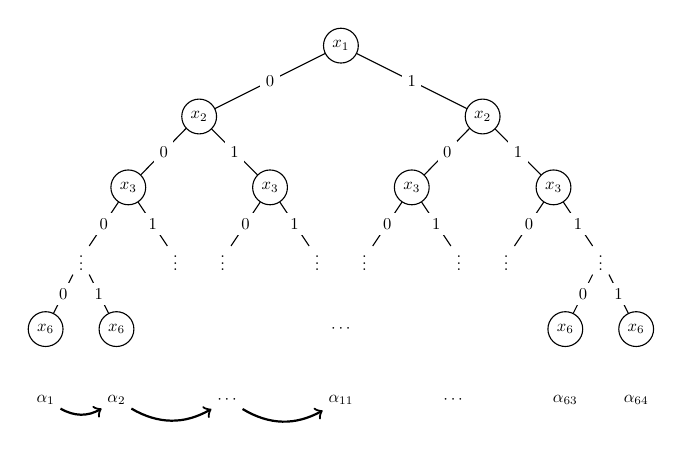
\begin{tikzpicture}[level/.style={sibling distance=60mm/#1},every node/.style={scale=0.6}, scale=0.6]
  \tikzstyle{trans}=[thick, ->, sloped]

\node [circle,draw] (x1) {$x_1$}
  child {node [circle,draw] (x2_1) {$x_2$}
    child {node [circle,draw] (x3_1) {$x_3$}
      child {node  (xn_1) {$\vdots$}
        child {node [circle,draw] (x6_1) {$x_6$}
         child { node (a1) {$\alpha_1$} edge from parent[draw=none]}}
        child {node [circle,draw] (x6_2) {$x_6$}
        	child { node (a2) {$\alpha_2$} edge from parent[draw=none]}}
      } 
      child {node (xn_2) {$\vdots$}}
    }
    child {node [circle,draw] (x3_2) {$x_3$}
      child {node (xn_3) {$\vdots$}}
      child {node (xn_4) {$\vdots$}}
    }
  }
  child {node [circle,draw] (x2_2) {$x_2$}
    child {node [circle,draw] (x3_3) {$x_3$}
      child {node (xn_5) {$\vdots$}}
      child {node (xn_6) {$\vdots$}}
    }
  child {node [circle,draw] (x3_4) {$x_3$}
    child {node (xn_7) {$\vdots$}}
    child {node (xn_8) {$\vdots$}
      child {node [circle,draw] (x6_3) {$x_6$}
        child { node (an_1) {$\alpha_{63}$} edge from parent[draw=none]}}
      child {node [circle,draw] (x6_4) {$x_6$}
        child { node (an) {$\alpha_{64}$} edge from parent[draw=none]}}
      }
  }
};

\path (x6_2) -- (x6_3) node (x) [midway] {$\cdots$}
        child { node (a_11) {$\alpha_{11}$} edge from parent[draw=none]};


\path (a2) -- (a_11) node (b1) [midway] {$\cdots$};
\path (a_11) -- (an_1) node (b2) [midway] {$\cdots$};

\draw[trans] (a1) to [bend right]  (a2);
\draw[trans] (a2) to [bend right]  (b1);
\draw[trans] (b1) to [bend right]  (a_11);

% to [bend right]  (b1) to [bend right]  (a_11);

\path (x1)   -- (x2_1) node [midway, fill=white] {$0$};
\path (x2_1) -- (x3_1) node [midway, fill=white] {$0$};
\path (x3_1) -- (xn_1) node [midway, fill=white] {$0$};
\path (xn_1) -- (x6_1) node [midway, fill=white] {$0$};
\path (x3_2) -- (xn_3) node [midway, fill=white] {$0$};
\path (x2_2) -- (x3_3) node [midway, fill=white] {$0$};
\path (x2_2) -- (x3_4) node [midway, fill=white] {$1$};
\path (x1)   -- (x2_2) node [midway, fill=white] {$1$};
\path (xn_1) -- (x6_2) node [midway, fill=white] {$1$};
\path (x3_1) -- (xn_2) node [midway, fill=white] {$1$};
\path (x2_1) -- (x3_2) node [midway, fill=white] {$1$};
\path (x3_2) -- (xn_4) node [midway, fill=white] {$1$};
\path (x3_3) -- (xn_5) node [midway, fill=white] {$0$};
\path (x3_3) -- (xn_6) node [midway, fill=white] {$1$};
\path (x3_4) -- (xn_7) node [midway, fill=white] {$0$};
\path (x3_4) -- (xn_8) node [midway, fill=white] {$1$};
\path (xn_8) -- (x6_3) node [midway, fill=white] {$0$};
\path (xn_8) -- (x6_4) node [midway, fill=white] {$1$};

\end{tikzpicture}
\end{minipage}
\begin{minipage}[c]{0.23\linewidth}
           \footnotesize
		\begin{itemize}
			\item[] $\omega_1 = \{x_1, x_2, x_3\}$ 
			\item[] $\omega_2 = \{x_4, x_5, x_6\}$
			\item[] $\omega_3 = \{\neg x_1, \neg x_5\}$
			\item[] $\omega_4 = \{\neg x_2, \neg x_4\}$
			\item[] $\omega_5 = \{\neg x_3, \neg x_4\}$
			\item[] $\omega_6 = \{\neg x_3, \neg x_6\}$
		\end{itemize}
\end{minipage}
